\documentclass{article}

% Styling.
\usepackage[margin = 1.4in]{geometry}
\usepackage[colorlinks = true, linkcolor = blue, citecolor = blue, urlcolor = black]{hyperref}

% Import packages.
\usepackage{bbm}
\usepackage{amsmath}
\usepackage{amsthm}
\usepackage{amssymb}
\usepackage{float}

% Import tikz libraries.
\usepackage{tikz}
\usepackage{pgfplots}
\usetikzlibrary{calc}
\pgfplotsset{compat=1.18}

% Create environments.
\newtheorem{theorem}{Theorem}
\newtheorem{corollary}[theorem]{Corollary}
\newtheorem{proposition}[theorem]{Proposition}
\newtheorem{lemma}[theorem]{Lemma}
\newtheorem{assumption}[theorem]{Assumption}
\theoremstyle{definition}
\newtheorem{definition}[theorem]{Definition}
\newtheorem{example}[theorem]{Example}
\newtheorem{conjecture}[theorem]{Conjecture}
\theoremstyle{remark}
\newtheorem*{remark}{Remark}

% Define commands.
\renewcommand{\leq}{\leqslant}
\renewcommand{\geq}{\geqslant}
\renewcommand{\epsilon}{\varepsilon}
\newcommand{\todo}[1]{\textcolor{red}{TODO: #1}}
\newcommand{\face}{\text{face}}
\newcommand{\ones}{\mathbbm1}
\newcommand{\tr}[1]{\textup{tr}\left(#1\right)}

% BibTex imports.
\usepackage{biblatex}
\addbibresource{./references.bib}

\begin{document}
Let $\Omega$ be a Lipschitz domain in $\mathbb R^m$ and let $\sigma\in L^\infty(\Omega)$ with $\text{essinf}(\sigma)>0$.
In the pioneering paper \cite{calderonpioneer} Calder\'on proposed the following question: is it possible to recover the function $\sigma$ from boundary measurements of solutions of the differential equation $-\text{div}(\sigma\nabla u)=0$?
As it was shown later, the answer to the question is affirmative if the Neumann-to-Dirichlet operator $\Lambda(\sigma)$ is known.
That is, if $u|_{\partial\Omega}$ is known for each $u$ solution of
\begin{equation}
\begin{cases}
-\text{div}(\sigma\nabla u)=0,\\
\sigma\frac{\partial u}{\partial n} = g,
\end{cases}
\end{equation}
with $g$ varying over $L^2_0(\partial\Omega)$.
The problem is, however, ill-posed in the sense of Hadamard, which makes it difficult to design reconstruction numerical schemes.
In \cite{convexcalderon} it was shown that if $\sigma$ is restricted to a suitable finite dimensional space of $L^\infty(\Omega)$ then the reconstruction can be obtained as the solution of a convex optimization problem.

Suppose that $\Omega$ is divided into $J$ disjoint pixels (connected open sets with Lipschitz boundary) $P_1,\dots,P_J$, $\overline\Omega = \bigcup_{j=1}^J \overline{P}_j$.
Throughout this work we assume the following:
\begin{assumption}\label{as:labeling}
The pixels are enumerated according to their distance to the boundary so that for each $j=1,\dots,J$ the set $\overline\Omega \setminus \left(\overline P_{j+1}\cup\cdots\cup \overline P_J\right)$ is connected and contains a non-empty open subset of $\partial\Omega$.
\end{assumption}
We identify a vector $\sigma\in\mathbb R^J_+$ with a conductivity by setting $\sigma(x) := \sum_j \sigma(j) \chi_{P_j}(x)$ and will usually restrict ourselves to $\sigma$ belonging to the compact set $K = [a,b]^J$ for some fixed $b>a>0$.
For $\sigma$ as described above, let $\Lambda(\sigma) \in L(L_0^2(\partial\Omega))$ be the Neumann-to-Dirichlet map associated to the differential expression $-\text{div}(\sigma\nabla u)=0$.
One of the main results in \cite{convexcalderon} stating that $\sigma$ can be characterized as the corner of certain convex set is shown below.

\begin{theorem}\label{thm:important}
There exists $c\in\mathbb R^J_+$ such that for all $\sigma\in K$ the optimization problem
\begin{align}
& \textup{min}\;\; c\tau \nonumber \\
& \textup{subject to }\; \tau \in K \label{eq:optimization} \\
& \phantom{\textup{subject to }\;} \Lambda(\tau) \leq \Lambda(\sigma) \nonumber
\end{align}
has $\sigma$ as the unique minimizer.
\end{theorem}

In this work we study the structure of the feasible set $\left\{\tau\in K: \Lambda(\tau)\leq\Lambda(\sigma)\right\}$ for a given $\sigma$ and then use that to conclude information about the weight vector $c$.
We start by recalling well-known facts about Calder\'on's map $\sigma\mapsto\Lambda(\sigma)$.

\begin{lemma}\label{lm:harrach}
Let $\Lambda:\mathbb R^J_+ \to L(L^2_0(\partial\Omega))$ be the Calder\'on's map.
The following holds:
\begin{enumerate}
\item $\Lambda(\sigma)$ is a self-adjoint positive semi-definite compact operator for each $\sigma\in\mathbb R^J_+$.\label{it:selfadjointness}
\item $\Lambda$ is monotonically decreasing. That is, if $\tau\geq\sigma$ component-wise then $\Lambda(\tau)\leq\Lambda(\sigma)$.
In particular $\Lambda'(\sigma)(e_j)\leq0$ for $j=1,\dots,J$.\label{it:monotonicity}
\item $\Lambda$ is convex, and in particular for $\tau,\sigma\in\mathbb R^J_+$ it holds that $\Lambda(\tau)-\Lambda(\sigma)\geq \Lambda'(\sigma)(\tau-\sigma)$.\label{it:convexity}
\item For any $\sigma\in\mathbb R^J_+$, $j\in \{1,2,\dots,J\}$ and constants $d_{j+1},\dots,d_J\in\mathbb R$ the operator
$$\Lambda'(\sigma)\left(e_j + d_{j+1}e_{j+1}+ \dots + d_J e_J\right)$$
is not positive semi-definite.\label{it:localizedpotentials}
\end{enumerate}
\end{lemma}
\begin{proof}
See \cite{convexcalderon}.
\end{proof}

\section*{Construction of Weights}
In this section we explore properties of the feasible set and their implications in terms of the weight vector $c$.

\begin{lemma}\label{lm:positivity}
Let $\sigma,\tau\in \mathbb R^J_+$ such that $\Lambda(\tau)\leq\Lambda(\sigma)$.
If $\sigma\neq\tau$ and $j\in\{1,2,\dots,J\}$ is the first component where they differ then $\tau(j) > \sigma(j)$.
\end{lemma}
\begin{proof}
Suppose by contradiction that $\delta = \tau(j) - \sigma(j) < 0$.
By convexity of $\Lambda$ in the form of part \ref{it:convexity} in Lemma \ref{lm:harrach} we have
\begin{align*}
\Lambda(\tau) - \Lambda(\sigma) &\geq \Lambda'(\sigma)(\tau-\sigma) \\
&= \Lambda'(\sigma)\left(\delta e_j + \sum_{k>j}(\tau(k)-\sigma(k))e_k \right) \\
&\not\leq 0
\end{align*}
where the last assertion follows from a localized potentials result as in part \ref{it:localizedpotentials} of Lemma \ref{lm:harrach}.
Therefore, we have reached a contradiction $\Lambda(\tau)-\Lambda(\sigma) \not\leq0$ from what follows $\tau(j)\geq \sigma(j)$.
\end{proof}
\begin{corollary}\label{cr:coordinate}
Let $\sigma\in K$ and $j\in\{1,2,\dots,J\}$.
If $\tau\in K$ is defined by
$$
\tau(k) = \begin{cases}
\sigma(k) &\text{ if }k\leq j, \\
b &\text{ otherwise},
\end{cases}
$$
then $\Lambda(\tau)\leq\Lambda(\sigma)$ and $\Lambda(\tau - \delta e_j) \not\leq \Lambda(\sigma)$ for any $0<\delta<\sigma(j)$.
\end{corollary}
\begin{proof}
The first part follows by monotonicity (Lemma \ref{lm:harrach} part \ref{it:monotonicity}) of the map $\Lambda$ since $\tau\geq\sigma$ while the second follows directly from Lemma \ref{lm:positivity}.
\end{proof}
Corollary \ref{cr:coordinate} says that, given the measurement $\Lambda(\sigma)$, one possible algorithm for recovering $\sigma$ is to start with the conductivity $\tau = b\ones$ and decrease one component at a time until $\tau$ is out of the feasibility region $\Lambda(\tau)\leq \Lambda(\sigma)$.
It is important to note that care should be taken when approximating $\Lambda(\tau)$ by a finite-dimensional projection as the boundary conditions used to show part \ref{it:localizedpotentials} in Lemma \ref{lm:harrach} may have arbitrarily large oscillations (see Figure \ref{fig:twodimensional}).
That is, for an unfeasible $\tau$ the boundary condition $f$ witnessing $\Lambda(\tau)\not\leq\Lambda(\sigma)$ (i.e. $ \langle\Lambda(\tau)f,f\rangle > \langle\Lambda(\sigma)f,f\rangle $) may not be in the space spanned by the chosen basis.
The result can be improved as shown below.
\begin{figure}[H]
\centering
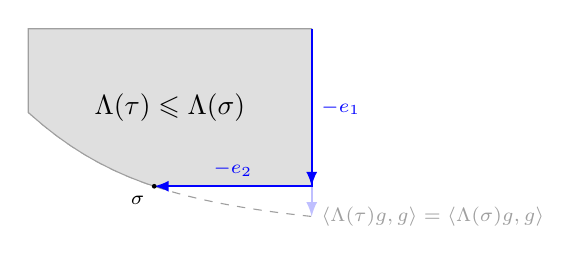
\begin{tikzpicture}[scale = 2, >=latex]
\draw[domain=0.2:2, smooth, variable=\x, dashed, gray!75] plot ({\x}, {
(-(5*\x-5)+sqrt((5*\x-5)^2+36*\x))/6
});
\draw[domain=0.2:1, smooth, variable=\x, gray!75, fill = gray!25] plot ({\x}, {
(-(5*\x-5)+sqrt((5*\x-5)^2+36*\x))/6
}) -- (2,1) -- (2,2) -- (0.2,2) -- cycle;
\draw[blue!25, thick, ->] (2,2) -- (2,0.808);
\node at (1.1,1.5) {$\Lambda(\tau)\leq\Lambda(\sigma)$};
\node[anchor = west, gray!75] at (2,0.808) {\scriptsize $ \langle\Lambda(\tau)g,g\rangle = \langle\Lambda(\sigma)g,g\rangle$};
\node[anchor = west, blue] at (2,1.5) {\scriptsize $-e_1$};
\node[anchor = south, blue] at (1.5,1) {\scriptsize $-e_2$};
\draw[blue, thick, ->] (2,2) -- (2,1);
\draw[blue, thick, ->] (2,2) -- (2,1) -- (1,1);
\fill[black] (1,1) circle (0.015);
\node[anchor = north east] at (1,1) {\scriptsize $\sigma$};
\end{tikzpicture}
\caption{Two-dimensional example of the feasible region and a low oscillating function $g$.}
\label{fig:twodimensional}
\end{figure}

We say that $P_j$ is adjacent to $P_k$ if $j\neq k$ and $\overline P_j \cap \overline P_k$ is a non-empty open relative set in $\partial P_j\cup \partial P_k$.
This relation defines a graph $G$ with vertices $P_1,\dots,P_J$ with a distinguished set $\partial G := \{ P_j : P_j \text{ touches }\partial\Omega\}$.
\begin{corollary}\label{cr:multipledescent}
Let $\sigma\in K$ and let $d:\{1,\dots,J\}\to\mathbb N$ defined by $d(j)=1+\textup{dist}_G(P_j,\partial G)$.
Then, for each $1\leq l \leq \max_j d(j)$, any minimizer $\tau$ of
\begin{align*}
&\textup{min}\;\; \sum_{j\in d^{-1}\left(\{l\}\right)}\tau(j) \\
&\textup{subject to }\; \tau \in K \\
&\phantom{\textup{subject to }\;} \Lambda(\tau) \leq \Lambda(\sigma) \\
&\phantom{\textup{subject to }\;} \tau(k) = \sigma(k) \textup{ if } d(k) < l
\end{align*}
satisfies $\tau(j)=\sigma(j)$ for each $j$ with $d(j)=l$.
\end{corollary}
\begin{proof}
Fix $\displaystyle l\leq 1$ and let $j$ such that $d(j)=l$.
If necessary relabel $P_1,\dots,P_J$ in such a way that $P_j$ comes as the $l$-th element and Assumption \ref{as:labeling} is satisfied.
Then it follows that $d(k)=k$ for $k<l$ and therefore, any $\tau$ in the feasible satisfies $\tau(k)=\sigma(k)$ for $k<l$.
Therefore, Lemma \ref{lm:positivity} implies that $\tau(j)\geq\sigma(j)$ for each $j$ with $d(j)=l$, and the assertion follows.
\end{proof}
Corollary \ref{cr:multipledescent}, as Corollary \ref{cr:coordinate}, provides an algorithm for recovering $\sigma$ by descending a group of coordinates at a time according to their distance to the boundary.
\begin{example}\label{ex:ones}
Let $\Omega = B_1(0)\subseteq \mathbb R^2$ and $P_j =\left\{ x\in \Omega : 0 < \|x\| < 1 \text{ and } \frac{2\pi(j-1)}{6} < \arg(x) < \frac{2\pi j}{6} \right\}$ for $j=1,\dots,J$ with $J=6$.
Note that $d(j)=1$ for each $j=1,\dots,J$ (i.e. each pixel $P_j$ touches the boundary) and therefore Corollary \ref{cr:multipledescent} implies that the weight vector $c$ can be chosen as $c = \ones$.
An interior-point method for solving problem \ref{eq:optimization} can be implemented as described below.
For each $\tau\in K$ let $\hat\Lambda(\tau)$ be a Galerkin projection of $\Lambda(\tau)$ with respect to the set $\left\{ \sin(k\theta),\cos(k\theta)\right\}_{k=1}^{n_b}$ for some $n_b\in\mathbb N$.
We consider the barrier function given by
$$ B(\tau) = -\sum_j\log(b-\tau_j) -\sum_j\log(\tau_j-a) - \log(\det(Y-\hat\Lambda(\tau))) $$
where $Y = \hat\Lambda(\sigma)$ is the measurement associated to the unknown conductivity $\sigma$.
The first two terms in the definition of $B$ guarantee that $\tau$ stays within $K =[a,b]^J$ while the last term guarantees that $\hat\Lambda(\tau)\leq\hat\Lambda(\sigma)$.
For each $t>0$ we consider the (in principle unbounded) optimization problem
\begin{align}
\min_{\tau\in\mathbb R^J_+}\;\; t\sum_j \tau(j) + B(\tau). \label{eq:interiorpoint}
\end{align}
We take $t\to\infty$, and for each fixed $t$ we approximate the solution to \eqref{eq:interiorpoint} by a simple gradient-descent scheme.
That is, if $f_t$ is the objective function in \eqref{eq:interiorpoint}, we update the iterates $\{\tau_n\}_n$ following the rule $\tau_{n+1}=\tau_n - \alpha \nabla f_t(\tau_n)$ where the step-size depends on $t$ and possibly on $n$.
A straightforward computations yields
$$
\partial_j f_t(\tau) = -\frac{1}{\tau(j)-b} - \frac{1}{\tau(j)-a} - \tr{(Y-\hat\Lambda(\tau))^{-1}\hat\Lambda'(\tau)(e_j)}
$$
where $\Lambda'(\tau)$ (and therefore $\hat\Lambda'(\tau)$) can be computed using the fact that
$$
\int_{\partial\Omega}g\Lambda'(\tau)(d)h\,\text ds = -\int_\Omega d(x)\nabla u^g(x) \cdot \nabla u^h(x) \,\text dx
$$
where $u^g$ and $u^h$ solve $-\text{div}(\tau\nabla u) = 0$ with Neumann boundary conditions $g$ and $h$ respectively.
A FreeFEM++ \cite{freefem} implementation can be found in this \href{https://github.com/jcvillaquira/convex-calderon}{repository}.
If $\{t_n\}_n$ is chosen geometrically increasing by $t_0=0$, $t_1=1.5$ and $t_{n+1} = 1.01 t_n$ and for each $n$ ten gradient descent steps are applied, then the error by epoch decreases as shown in Figure \ref{fig:convexerror}.
\begin{figure}[H]
\centering
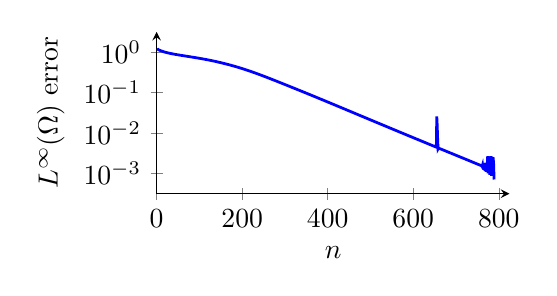
\begin{tikzpicture}
    \begin{axis}[axis lines = left, xmin = 0, xmax = 825, ymax = 0.5, ymin = -3.5, width = .5\linewidth, height = 0.3\linewidth, xlabel = {$n$}, ylabel = {$L^\infty(\Omega)$ error}, legend cell align={left}, legend columns={1}, yticklabels={{$10^0$,$10^{-1}$,$10^{-2}$,$10^{-3}$}}, ytick={{0,-1,-2,-3}}, xtick={{0,200,400,600,800}}]
    \addplot[color=blue, draw opacity={1.0}, line width={1}, solid]
        table[row sep={\\}]
        {
            \\
            1.0  0.08416701454464202  \\
            2.0  0.07228503959816909  \\
            3.0  0.06571620563659901  \\
            4.0  0.059663959379244735  \\
            5.0  0.05402884106966033  \\
            6.0  0.04875073702650333  \\
            7.0  0.04377694611658174  \\
            8.0  0.03907113597795089  \\
            9.0  0.03459459690867442  \\
            10.0  0.03033071094800073  \\
            11.0  0.026249457532898902  \\
            12.0  0.022339922553213674  \\
            13.0  0.018586322169304174  \\
            14.0  0.014972057305417093  \\
            15.0  0.01148821474535504  \\
            16.0  0.008125410435444957  \\
            17.0  0.00486951470336307  \\
            18.0  0.0017188182113785757  \\
            19.0  -0.0013329095502209894  \\
            20.0  -0.004296566287064594  \\
            21.0  -0.007179021766532298  \\
            22.0  -0.009978514896159566  \\
            23.0  -0.01271119581765578  \\
            24.0  -0.015371182823890276  \\
            25.0  -0.017966079927845338  \\
            26.0  -0.02049916933776521  \\
            27.0  -0.02297385203038386  \\
            28.0  -0.025398248932525284  \\
            29.0  -0.027771434681693397  \\
            30.0  -0.03009249144623449  \\
            31.0  -0.03236986784374857  \\
            32.0  -0.03460751136121866  \\
            33.0  -0.036800016231699914  \\
            34.0  -0.0389608888110619  \\
            35.0  -0.04108005180637488  \\
            36.0  -0.043166432836018696  \\
            37.0  -0.04522432708730394  \\
            38.0  -0.04724843808138633  \\
            39.0  -0.04924797464518652  \\
            40.0  -0.05121766575345986  \\
            41.0  -0.05316197021779518  \\
            42.0  -0.055080505556173734  \\
            43.0  -0.056982793884888194  \\
            44.0  -0.05885863689330658  \\
            45.0  -0.06071764357951372  \\
            46.0  -0.06255956206845882  \\
            47.0  -0.06437910328136082  \\
            48.0  -0.06618606773888171  \\
            49.0  -0.06798026599963738  \\
            50.0  -0.06975640836250646  \\
            51.0  -0.07151936241523389  \\
            52.0  -0.07327407844051713  \\
            53.0  -0.07501526534679648  \\
            54.0  -0.07674273127431816  \\
            55.0  -0.07846668982734012  \\
            56.0  -0.08017662455123165  \\
            57.0  -0.08188283013700484  \\
            58.0  -0.08357997126440715  \\
            59.0  -0.08527320009393162  \\
            60.0  -0.08695713899103769  \\
            61.0  -0.0886369800133882  \\
            62.0  -0.09031265005423396  \\
            63.0  -0.09198944295119443  \\
            64.0  -0.09365657018098214  \\
            65.0  -0.09532471275013124  \\
            66.0  -0.09698842797755916  \\
            67.0  -0.09865309061156426  \\
            68.0  -0.10031321558819953  \\
            69.0  -0.10197421849373735  \\
            70.0  -0.10363608502306514  \\
            71.0  -0.1052988006729935  \\
            72.0  -0.1069623507403129  \\
            73.0  -0.10862672031983711  \\
            74.0  -0.11029189430243584  \\
            75.0  -0.11196347748516203  \\
            76.0  -0.11363023573129746  \\
            77.0  -0.11530907897617684  \\
            78.0  -0.11698306616896051  \\
            79.0  -0.11866353071696012  \\
            80.0  -0.1203505229421377  \\
            81.0  -0.1220383416670646  \\
            82.0  -0.12373274544003689  \\
            83.0  -0.12543378584569  \\
            84.0  -0.12714151507718402  \\
            85.0  -0.1288501429257733  \\
            86.0  -0.13056551952236978  \\
            87.0  -0.1322876983909389  \\
            88.0  -0.13402264664193322  \\
            89.0  -0.13575861687616958  \\
            90.0  -0.13750155402151215  \\
            91.0  -0.1392515142235046  \\
            92.0  -0.14100855430914375  \\
            93.0  -0.14277876516934448  \\
            94.0  -0.14455016294362996  \\
            95.0  -0.14633489846243836  \\
            96.0  -0.14812699863699974  \\
            97.0  -0.14992652449929464  \\
            98.0  -0.15173353784313298  \\
            99.0  -0.15355428617708666  \\
            100.0  -0.15538270001563614  \\
            101.0  -0.1572188441766125  \\
            102.0  -0.15906904828152202  \\
            103.0  -0.16092716845938623  \\
            104.0  -0.16279327273898914  \\
            105.0  -0.16467377537007266  \\
            106.0  -0.16656245603398667  \\
            107.0  -0.1684657871579889  \\
            108.0  -0.17037749651824927  \\
            109.0  -0.17229765820099727  \\
            110.0  -0.174232833831479  \\
            111.0  -0.1761766710332937  \\
            112.0  -0.17813579279931568  \\
            113.0  -0.18010379231399248  \\
            114.0  -0.1820873553348572  \\
            115.0  -0.18408001951183076  \\
            116.0  -0.18608186874745977  \\
            117.0  -0.1881063822239325  \\
            118.0  -0.1901336488717284  \\
            119.0  -0.19217718328296124  \\
            120.0  -0.19423037884286753  \\
            121.0  -0.19630015199540077  \\
            122.0  -0.19838669411531834  \\
            123.0  -0.20048330931828925  \\
            124.0  -0.20259009533483524  \\
            125.0  -0.2047141094932114  \\
            126.0  -0.20684856269257454  \\
            127.0  -0.20900058523583767  \\
            128.0  -0.21116332463993506  \\
            129.0  -0.2133439859933134  \\
            130.0  -0.21553565207230782  \\
            131.0  -0.21774560462985934  \\
            132.0  -0.21996686030201365  \\
            133.0  -0.22219953530618916  \\
            134.0  -0.2244510293433215  \\
            135.0  -0.2267142565575078  \\
            136.0  -0.2289966981768051  \\
            137.0  -0.2312911986078428  \\
            138.0  -0.23359788594821054  \\
            139.0  -0.2359243669611832  \\
            140.0  -0.23826337789992777  \\
            141.0  -0.24062261239744268  \\
            142.0  -0.2429947330886301  \\
            143.0  -0.24642799597432183  \\
            144.0  -0.2488013193018576  \\
            145.0  -0.2511954278030447  \\
            146.0  -0.25361059472495123  \\
            147.0  -0.25603143679837026  \\
            148.0  -0.2584737238580849  \\
            149.0  -0.26093774287993693  \\
            150.0  -0.26341582160052446  \\
            151.0  -0.26590812139042136  \\
            152.0  -0.2684148064144475  \\
            153.0  -0.27094414816260415  \\
            154.0  -0.2734883071977065  \\
            155.0  -0.2760474581473086  \\
            156.0  -0.2786300279136114  \\
            157.0  -0.2812197484072088  \\
            158.0  -0.2838333528193568  \\
            159.0  -0.28646278130258623  \\
            160.0  -0.28910822663840025  \\
            161.0  -0.2917698851528327  \\
            162.0  -0.2944479568038772  \\
            163.0  -0.2971512538464993  \\
            164.0  -0.29986282054233476  \\
            165.0  -0.30260014089764076  \\
            166.0  -0.3053460511081211  \\
            167.0  -0.3081094333920082  \\
            168.0  -0.3108993969682576  \\
            169.0  -0.3136984564941002  \\
            170.0  -0.3165156732501159  \\
            171.0  -0.319351284343649  \\
            172.0  -0.3222055315570066  \\
            173.0  -0.32507866147117115  \\
            174.0  -0.32797092559363406  \\
            175.0  -0.33087327665036864  \\
            176.0  -0.3338045210741998  \\
            177.0  -0.33674625376007367  \\
            178.0  -0.33969855366678464  \\
            179.0  -0.3426806205705948  \\
            180.0  -0.34567367900389717  \\
            181.0  -0.34868750814244054  \\
            182.0  -0.35171263711486184  \\
            183.0  -0.35475898587199667  \\
            184.0  -0.35782685421061505  \\
            185.0  -0.3609065783096407  \\
            186.0  -0.3640082978081061  \\
            187.0  -0.367122215414522  \\
            188.0  -0.3702586213374481  \\
            189.0  -0.3734075815833608  \\
            190.0  -0.37657954101217606  \\
            191.0  -0.3797644255829696  \\
            192.0  -0.38297283905668184  \\
            193.0  -0.3861913935939235  \\
            194.0  -0.3894286556711824  \\
            195.0  -0.39268379377191603  \\
            196.0  -0.3959559486785843  \\
            197.0  -0.39924532154217174  \\
            198.0  -0.4025521172143197  \\
            199.0  -0.40587433282507307  \\
            200.0  -0.40921435826176383  \\
            201.0  -0.4125712864271216  \\
            202.0  -0.4159441792547637  \\
            203.0  -0.41933434780689766  \\
            204.0  -0.42274084286617336  \\
            205.0  -0.4261638411062466  \\
            206.0  -0.4296035222243304  \\
            207.0  -0.4330588918293567  \\
            208.0  -0.4365301075299687  \\
            209.0  -0.44001732944677635  \\
            210.0  -0.44352192615168246  \\
            211.0  -0.4470404453030462  \\
            212.0  -0.4505754469138799  \\
            213.0  -0.45412710133504014  \\
            214.0  -0.4576930899372084  \\
            215.0  -0.46127478299382996  \\
            216.0  -0.464871060607384  \\
            217.0  -0.4684833171667079  \\
            218.0  -0.4721104154227816  \\
            219.0  -0.47575117696457864  \\
            220.0  -0.47940831018570235  \\
            221.0  -0.4830793295444404  \\
            222.0  -0.4867643260273238  \\
            223.0  -0.4904633912830103  \\
            224.0  -0.49417661762293313  \\
            225.0  -0.49790409802170876  \\
            226.0  -0.5016445475449876  \\
            227.0  -0.5053994151204008  \\
            228.0  -0.509167392599276  \\
            229.0  -0.5129485383350445  \\
            230.0  -0.5167429104128661  \\
            231.0  -0.5205505666240163  \\
            232.0  -0.5243701118087979  \\
            233.0  -0.5282030299610916  \\
            234.0  -0.5320478988071726  \\
            235.0  -0.5359032428907976  \\
            236.0  -0.5397720471584191  \\
            237.0  -0.5436528464455771  \\
            238.0  -0.54754412034066  \\
            239.0  -0.5514473836640781  \\
            240.0  -0.5553626445014473  \\
            241.0  -0.5592867607191596  \\
            242.0  -0.5632228280226832  \\
            243.0  -0.567169244992644  \\
            244.0  -0.5711259673040563  \\
            245.0  -0.5750929475543152  \\
            246.0  -0.5790701351661554  \\
            247.0  -0.5830558134844197  \\
            248.0  -0.5870515573394652  \\
            249.0  -0.5910573054780267  \\
            250.0  -0.5950712835987827  \\
            251.0  -0.5990933754061343  \\
            252.0  -0.6031252011203676  \\
            253.0  -0.6071649255611596  \\
            254.0  -0.6112124177990292  \\
            255.0  -0.6152693323932054  \\
            256.0  -0.6193319627841098  \\
            257.0  -0.6234037604635567  \\
            258.0  -0.627482782030475  \\
            259.0  -0.6315688689809126  \\
            260.0  -0.6356618567273553  \\
            261.0  -0.6397615744383215  \\
            262.0  -0.643867844874872  \\
            263.0  -0.6479804842240491  \\
            264.0  -0.6520993019292485  \\
            265.0  -0.6562241005175471  \\
            266.0  -0.6603546754240027  \\
            267.0  -0.6644908148129588  \\
            268.0  -0.6686322993963884  \\
            269.0  -0.6727789022493195  \\
            270.0  -0.6769303886223951  \\
            271.0  -0.6810865157516265  \\
            272.0  -0.6852491366007818  \\
            273.0  -0.6894138041969267  \\
            274.0  -0.693584479146565  \\
            275.0  -0.697758781382808  \\
            276.0  -0.7019386121336623  \\
            277.0  -0.7061215330067641  \\
            278.0  -0.7103072409042566  \\
            279.0  -0.7144976736163813  \\
            280.0  -0.7186925740842547  \\
            281.0  -0.7228893821376985  \\
            282.0  -0.7270900729658226  \\
            283.0  -0.7312920228803619  \\
            284.0  -0.7354995938707332  \\
            285.0  -0.7397077809181393  \\
            286.0  -0.7439210178102813  \\
            287.0  -0.7481366195557542  \\
            288.0  -0.7523542529993643  \\
            289.0  -0.7565735745854701  \\
            290.0  -0.7607967338208701  \\
            291.0  -0.7650209109211169  \\
            292.0  -0.7692482834015703  \\
            293.0  -0.7734759616394413  \\
            294.0  -0.7777087543691098  \\
            295.0  -0.781941148088015  \\
            296.0  -0.7861753774197482  \\
            297.0  -0.7904137688041388  \\
            298.0  -0.7946533295667342  \\
            299.0  -0.7988936844832203  \\
            300.0  -0.8031344469512962  \\
            301.0  -0.8073780059134866  \\
            302.0  -0.8116240334130482  \\
            303.0  -0.8158721910595635  \\
            304.0  -0.8201192596470671  \\
            305.0  -0.8243705913000668  \\
            306.0  -0.8286229727427596  \\
            307.0  -0.8328760215436498  \\
            308.0  -0.8371293436786706  \\
            309.0  -0.8413855474709178  \\
            310.0  -0.8456443040516983  \\
            311.0  -0.8499022001477545  \\
            312.0  -0.8541618988946257  \\
            313.0  -0.8584230382468807  \\
            314.0  -0.8626852449385563  \\
            315.0  -0.8669513311840853  \\
            316.0  -0.8712145382314586  \\
            317.0  -0.8754808837902902  \\
            318.0  -0.8797500438946978  \\
            319.0  -0.8840183590170925  \\
            320.0  -0.8882887433855059  \\
            321.0  -0.8925608399196158  \\
            322.0  -0.896834280363229  \\
            323.0  -0.901108685045919  \\
            324.0  -0.9053871554114535  \\
            325.0  -0.9096623372585699  \\
            326.0  -0.9139408360317033  \\
            327.0  -0.9182223297892309  \\
            328.0  -0.9225028529093683  \\
            329.0  -0.9267856234019283  \\
            330.0  -0.9310702860424189  \\
            331.0  -0.9353564744027741  \\
            332.0  -0.9396400311804871  \\
            333.0  -0.9439319051026841  \\
            334.0  -0.9482203563889176  \\
            335.0  -0.9525126438955449  \\
            336.0  -0.9568045257311493  \\
            337.0  -0.9610995351045678  \\
            338.0  -0.9653933295130392  \\
            339.0  -0.9696894965464733  \\
            340.0  -0.9739876809684396  \\
            341.0  -0.9782875162670991  \\
            342.0  -0.9825927967052762  \\
            343.0  -0.9868906155983874  \\
            344.0  -0.9911973438019261  \\
            345.0  -0.9955042239472394  \\
            346.0  -0.999810830704933  \\
            347.0  -1.0041211103147578  \\
            348.0  -1.0084303147390168  \\
            349.0  -1.012746925389585  \\
            350.0  -1.017057182630008  \\
            351.0  -1.0213741494060549  \\
            352.0  -1.0256929881960462  \\
            353.0  -1.0300133221616854  \\
            354.0  -1.0343300624123155  \\
            355.0  -1.0386521615587465  \\
            356.0  -1.0429793474899667  \\
            357.0  -1.0473016530167107  \\
            358.0  -1.0516331690764031  \\
            359.0  -1.0559589172326824  \\
            360.0  -1.0602882661615036  \\
            361.0  -1.0646208884557573  \\
            362.0  -1.0689564458492118  \\
            363.0  -1.0732894476256534  \\
            364.0  -1.077629764085835  \\
            365.0  -1.081966687533454  \\
            366.0  -1.0863049734534669  \\
            367.0  -1.0906495748077962  \\
            368.0  -1.0949894330407741  \\
            369.0  -1.09933488190963  \\
            370.0  -1.1036801361337432  \\
            371.0  -1.1080303176558468  \\
            372.0  -1.1123795081308352  \\
            373.0  -1.1167329167283637  \\
            374.0  -1.121084488677708  \\
            375.0  -1.125439521660219  \\
            376.0  -1.129791821097959  \\
            377.0  -1.1341526891860385  \\
            378.0  -1.1385099926291369  \\
            379.0  -1.1428692118629447  \\
            380.0  -1.147229959588869  \\
            381.0  -1.1515979933567122  \\
            382.0  -1.155960648890933  \\
            383.0  -1.1603235968272185  \\
            384.0  -1.1646927447152422  \\
            385.0  -1.169061423725052  \\
            386.0  -1.1734356453612929  \\
            387.0  -1.177802048689257  \\
            388.0  -1.1821797649403953  \\
            389.0  -1.186555343071081  \\
            390.0  -1.1909282665444676  \\
            391.0  -1.1953048128853998  \\
            392.0  -1.1996846420617966  \\
            393.0  -1.2040674026604314  \\
            394.0  -1.2084457132959319  \\
            395.0  -1.212826074912069  \\
            396.0  -1.2172152594676369  \\
            397.0  -1.2215986150023042  \\
            398.0  -1.2259243605509764  \\
            399.0  -1.230323148553307  \\
            400.0  -1.2347222079538118  \\
            401.0  -1.239113557013422  \\
            402.0  -1.2435117190531577  \\
            403.0  -1.2479087603119006  \\
            404.0  -1.2523041885970174  \\
            405.0  -1.2567053401253845  \\
            406.0  -1.261104009594051  \\
            407.0  -1.2654996622907344  \\
            408.0  -1.2698998330202893  \\
            409.0  -1.2742960351903556  \\
            410.0  -1.2786959394956394  \\
            411.0  -1.283099201652292  \\
            412.0  -1.2875054657764755  \\
            413.0  -1.2919058587185854  \\
            414.0  -1.296308332481705  \\
            415.0  -1.3007124919797564  \\
            416.0  -1.3051179294171318  \\
            417.0  -1.3095242240108365  \\
            418.0  -1.3139309417114848  \\
            419.0  -1.3183376349235292  \\
            420.0  -1.3227438422250801  \\
            421.0  -1.3271490880877796  \\
            422.0  -1.3315622010079495  \\
            423.0  -1.3359735480575947  \\
            424.0  -1.3403826124665108  \\
            425.0  -1.3447984690161436  \\
            426.0  -1.3492111594118525  \\
            427.0  -1.3536201231035392  \\
            428.0  -1.3580346875458975  \\
            429.0  -1.3624445576210398  \\
            430.0  -1.3668592338438292  \\
            431.0  -1.3712784018475008  \\
            432.0  -1.3756914209753848  \\
            433.0  -1.3801080587112688  \\
            434.0  -1.3845279633465768  \\
            435.0  -1.3889401365074217  \\
            436.0  -1.3933653632014877  \\
            437.0  -1.3977818747143378  \\
            438.0  -1.4021999015548627  \\
            439.0  -1.4066190264334115  \\
            440.0  -1.4110388187899068  \\
            441.0  -1.4154588345102166  \\
            442.0  -1.4198786156419227  \\
            443.0  -1.424297690109868  \\
            444.0  -1.428715571431947  \\
            445.0  -1.4331435323793527  \\
            446.0  -1.437569523742742  \\
            447.0  -1.4419810012867456  \\
            448.0  -1.4464134704869163  \\
            449.0  -1.4508303230951078  \\
            450.0  -1.4552553889387856  \\
            451.0  -1.4596759404358528  \\
            452.0  -1.464104016495902  \\
            453.0  -1.4685266096751417  \\
            454.0  -1.4729430841977311  \\
            455.0  -1.4773658227505229  \\
            456.0  -1.4817945539137642  \\
            457.0  -1.4862156914499656  \\
            458.0  -1.4906419752767277  \\
            459.0  -1.4950730983030864  \\
            460.0  -1.4994950246751748  \\
            461.0  -1.5039208615974806  \\
            462.0  -1.5083362637573487  \\
            463.0  -1.51276873041352  \\
            464.0  -1.517189746177003  \\
            465.0  -1.5216129248843466  \\
            466.0  -1.5260378677594082  \\
            467.0  -1.5304641631157254  \\
            468.0  -1.5348913860721738  \\
            469.0  -1.5393190982674045  \\
            470.0  -1.543731658769875  \\
            471.0  -1.548112793334661  \\
            472.0  -1.5525540752452838  \\
            473.0  -1.5569942641730479  \\
            474.0  -1.561417034670624  \\
            475.0  -1.5658533439511306  \\
            476.0  -1.570270850787456  \\
            477.0  -1.5747011296692224  \\
            478.0  -1.5791276307624682  \\
            479.0  -1.5835497698366048  \\
            480.0  -1.5879669460433854  \\
            481.0  -1.5923955307852453  \\
            482.0  -1.5968182471436458  \\
            483.0  -1.6012517864751599  \\
            484.0  -1.6056609819344403  \\
            485.0  -1.6100977048514007  \\
            486.0  -1.6145087076330413  \\
            487.0  -1.6189288506662793  \\
            488.0  -1.6233579524126045  \\
            489.0  -1.6277773914950848  \\
            490.0  -1.6322050237138117  \\
            491.0  -1.6366218250654028  \\
            492.0  -1.6410459991035948  \\
            493.0  -1.6454581105962072  \\
            494.0  -1.6498767171702033  \\
            495.0  -1.6543015556931846  \\
            496.0  -1.6587125603975885  \\
            497.0  -1.663148830513555  \\
            498.0  -1.6675500803618213  \\
            499.0  -1.6719759840369022  \\
            500.0  -1.6763856094870189  \\
            501.0  -1.6808196414954637  \\
            502.0  -1.6852362902370823  \\
            503.0  -1.689655806863066  \\
            504.0  -1.6940563445987942  \\
            505.0  -1.6984802373080135  \\
            506.0  -1.7029058306401959  \\
            507.0  -1.7073105743907209  \\
            508.0  -1.7117380873174486  \\
            509.0  -1.716143425742936  \\
            510.0  -1.7205482645971926  \\
            511.0  -1.7249751824547328  \\
            512.0  -1.7293778161378353  \\
            513.0  -1.7338020100177678  \\
            514.0  -1.738224197443698  \\
            515.0  -1.7426198392873828  \\
            516.0  -1.747036169456117  \\
            517.0  -1.7514488606201986  \\
            518.0  -1.7558573375946487  \\
            519.0  -1.7602610088498403  \\
            520.0  -1.7646845275748064  \\
            521.0  -1.7691025224928822  \\
            522.0  -1.7734885780278766  \\
            523.0  -1.7779193818135268  \\
            524.0  -1.7823169227397662  \\
            525.0  -1.7867328692840903  \\
            526.0  -1.7911404783275664  \\
            527.0  -1.7955390311748998  \\
            528.0  -1.7999551887852472  \\
            529.0  -1.804361353237051  \\
            530.0  -1.8087567552115986  \\
            531.0  -1.8131688506588615  \\
            532.0  -1.8175691594777919  \\
            533.0  -1.8219856833492611  \\
            534.0  -1.8263893410227663  \\
            535.0  -1.8307792754140484  \\
            536.0  -1.8351843221126358  \\
            537.0  -1.8395744704346513  \\
            538.0  -1.8439791275369752  \\
            539.0  -1.8483982816208278  \\
            540.0  -1.8528009717073004  \\
            541.0  -1.857186230013395  \\
            542.0  -1.8615846422123694  \\
            543.0  -1.865996156026674  \\
            544.0  -1.8703884899595722  \\
            545.0  -1.8747931477969726  \\
            546.0  -1.8791771667496322  \\
            547.0  -1.883572674185739  \\
            548.0  -1.8879795671250104  \\
            549.0  -1.8923638394563085  \\
            550.0  -1.896758581403767  \\
            551.0  -1.9011636587599476  \\
            552.0  -1.9055789306936546  \\
            553.0  -1.9099689498524506  \\
            554.0  -1.9143681394973553  \\
            555.0  -1.91874030436246  \\
            556.0  -1.9231205479955094  \\
            557.0  -1.9275454207628202  \\
            558.0  -1.9319044464597044  \\
            559.0  -1.936307667785302  \\
            560.0  -1.940718100398546  \\
            561.0  -1.9450972318097581  \\
            562.0  -1.949482307432866  \\
            563.0  -1.9538730561891156  \\
            564.0  -1.9582691971193615  \\
            565.0  -1.962630588533852  \\
            566.0  -1.9670362238053838  \\
            567.0  -1.9714056779495819  \\
            568.0  -1.9758195405199606  \\
            569.0  -1.9801957285483558  \\
            570.0  -1.9845745466869105  \\
            571.0  -1.988955623768887  \\
            572.0  -1.9933385765623792  \\
            573.0  -1.9977230095011371  \\
            574.0  -2.0021085144137802  \\
            575.0  -2.006494670251752  \\
            576.0  -2.0108810428163095  \\
            577.0  -2.0152671844849372  \\
            578.0  -2.0196526339375436  \\
            579.0  -2.0240369158829163  \\
            580.0  -2.0284195407858294  \\
            581.0  -2.032800004595318  \\
            582.0  -2.0371777884746027  \\
            583.0  -2.0415523585332633  \\
            584.0  -2.0459231655621912  \\
            585.0  -2.0502896447719743  \\
            586.0  -2.0547004716503454  \\
            587.0  -2.059057033813084  \\
            588.0  -2.063407482053939  \\
            589.0  -2.0678019512833465  \\
            590.0  -2.0721900553487984  \\
            591.0  -2.076571143533622  \\
            592.0  -2.0809445476352253  \\
            593.0  -2.0853095817306766  \\
            594.0  -2.089665541951845  \\
            595.0  -2.0940656353474107  \\
            596.0  -2.098401804487435  \\
            597.0  -2.102781704662812  \\
            598.0  -2.1071506412809833  \\
            599.0  -2.111507829572791  \\
            600.0  -2.1159091760536715  \\
            601.0  -2.1202982906653087  \\
            602.0  -2.124616474909866  \\
            603.0  -2.1290364773117374  \\
            604.0  -2.133383824937268  \\
            605.0  -2.13777513050761  \\
            606.0  -2.142090798086984  \\
            607.0  -2.146510632638049  \\
            608.0  -2.1508529608651084  \\
            609.0  -2.1552391450760253  \\
            610.0  -2.1596073577243566  \\
            611.0  -2.1639565996504087  \\
            612.0  -2.1682858494988517  \\
            613.0  -2.1726586902267453  \\
            614.0  -2.1770107214519405  \\
            615.0  -2.1814068058695573  \\
            616.0  -2.185781225346454  \\
            617.0  -2.19013286470566  \\
            618.0  -2.194460585292444  \\
            619.0  -2.1988318658128923  \\
            620.0  -2.2031782499420984  \\
            621.0  -2.20756857243498  \\
            622.0  -2.2119329764613656  \\
            623.0  -2.2162702213150465  \\
            624.0  -2.220651219013949  \\
            625.0  -2.225003944977587  \\
            626.0  -2.229400738270985  \\
            627.0  -2.233693707341315  \\
            628.0  -2.238104672691805  \\
            629.0  -2.2424090890207276  \\
            630.0  -2.2468332569165708  \\
            631.0  -2.251148062298157  \\
            632.0  -2.2555061667069425  \\
            633.0  -2.2598294432102777  \\
            634.0  -2.264196189780813  \\
            635.0  -2.268607289478572  \\
            636.0  -2.272900799260318  \\
            637.0  -2.277319415714293  \\
            638.0  -2.2816172952463543  \\
            639.0  -2.28595813307659  \\
            640.0  -2.290342796638692  \\
            641.0  -2.294686572038997  \\
            642.0  -2.299074232807868  \\
            643.0  -2.303419327892391  \\
            644.0  -2.3077201189113254  \\
            645.0  -2.3120639267418706  \\
            646.0  -2.316451620599578  \\
            647.0  -2.3207931839508102  \\
            648.0  -2.3251785877591677  \\
            649.0  -2.329515969460497  \\
            650.0  -2.3338034294358985  \\
            651.0  -2.3382282547792737  \\
            652.0  -2.342507458127509  \\
            653.0  -2.346925775278984  \\
            654.0  -2.3511944726195426  \\
            655.0  -1.5910042697844333  \\
            656.0  -1.8078623641102767  \\
            657.0  -2.1316737157765555  \\
            658.0  -2.3939877993303966  \\
            659.0  -2.3757625399962476  \\
            660.0  -2.377519954408151  \\
            661.0  -2.3816833173815612  \\
            662.0  -2.385992593692387  \\
            663.0  -2.3903450575769014  \\
            664.0  -2.3947415834578325  \\
            665.0  -2.399074201402185  \\
            666.0  -2.403340532324484  \\
            667.0  -2.407427190324092  \\
            668.0  -2.4121131838263  \\
            669.0  -2.4163969049685114  \\
            670.0  -2.4207233004348443  \\
            671.0  -2.425093229028977  \\
            672.0  -2.429390832026711  \\
            673.0  -2.4337313877670557  \\
            674.0  -2.4381157635146344  \\
            675.0  -2.4424245521310084  \\
            676.0  -2.4467765184972334  \\
            677.0  -2.4511725367361623  \\
            678.0  -2.455489532297964  \\
            679.0  -2.459849871076137  \\
            680.0  -2.464127965745995  \\
            681.0  -2.468576353296898  \\
            682.0  -2.4728126956910033  \\
            683.0  -2.477221067795658  \\
            684.0  -2.4815430054298364  \\
            685.0  -2.4859083860755016  \\
            686.0  -2.490183804566544  \\
            687.0  -2.494501731298281  \\
            688.0  -2.498863020040613  \\
            689.0  -2.503268550546344  \\
            690.0  -2.5075794532805835  \\
            691.0  -2.511933576358457  \\
            692.0  -2.5161892197315403  \\
            693.0  -2.520630970718592  \\
            694.0  -2.5249731305731764  \\
            695.0  -2.529212226689521  \\
            696.0  -2.5336414801919553  \\
            697.0  -2.5379664640079063  \\
            698.0  -2.5423349524045373  \\
            699.0  -2.546594912530522  \\
            700.0  -2.5508970725445543  \\
            701.0  -2.555242276897371  \\
            702.0  -2.5596313956432684  \\
            703.0  -2.563906188888902  \\
            704.0  -2.568223477881274  \\
            705.0  -2.572584116012029  \\
            706.0  -2.576988982640247  \\
            707.0  -2.581273353593982  \\
            708.0  -2.585600411884267  \\
            709.0  -2.589971016709555  \\
            710.0  -2.5942154118231047  \\
            711.0  -2.5986740319681125  \\
            712.0  -2.6030047700769776  \\
            713.0  -2.607379129192057  \\
            714.0  -2.611620376333784  \\
            715.0  -2.615903451606663  \\
            716.0  -2.6202291882722015  \\
            717.0  -2.6245984447417623  \\
            718.0  -2.6290121055990574  \\
            719.0  -2.6332843750576544  \\
            720.0  -2.637599089850307  \\
            721.0  -2.641957101842932  \\
            722.0  -2.6463592888066834  \\
            723.0  -2.650612246124837  \\
            724.0  -2.65510350499163  \\
            725.0  -2.659443394119797  \\
            726.0  -2.6636268679632678  \\
            727.0  -2.6680532118567952  \\
            728.0  -2.6723208628525246  \\
            729.0  -2.676837176080194  \\
            730.0  -2.6811924613345495  \\
            731.0  -2.685381356896551  \\
            732.0  -2.6898236192199447  \\
            733.0  -2.6940970125792782  \\
            734.0  -2.698412873718869  \\
            735.0  -2.7027720551838486  \\
            736.0  -2.7071754354522457  \\
            737.0  -2.711623919997646  \\
            738.0  -2.715892608144084  \\
            739.0  -2.7204317579208106  \\
            740.0  -2.7245579556884554  \\
            741.0  -2.7291890727998065  \\
            742.0  -2.733399726404163  \\
            743.0  -2.737889044346037  \\
            744.0  -2.7421853208876152  \\
            745.0  -2.74652452352852  \\
            746.0  -2.7509075187224936  \\
            747.0  -2.7553351994246467  \\
            748.0  -2.7595587577877905  \\
            749.0  -2.7640759880779235  \\
            750.0  -2.768385840156662  \\
            751.0  -2.7727388914084683  \\
            752.0  -2.777136016610204  \\
            753.0  -2.7815781173817826  \\
            754.0  -2.7858008351871812  \\
            755.0  -2.79033292116515  \\
            756.0  -2.794371478056376  \\
            757.0  -2.799267847500519  \\
            758.0  -2.802838764420948  \\
            759.0  -2.8092293741818763  \\
            760.0  -2.8083904640924096  \\
            761.0  -2.8266484024661716  \\
            762.0  -2.7919438401262724  \\
            763.0  -2.884866533126306  \\
            764.0  -2.745073300131943  \\
            765.0  -2.9095418410349363  \\
            766.0  -2.7419455205851584  \\
            767.0  -2.92534175920526  \\
            768.0  -2.7397932554807225  \\
            769.0  -2.9406004379366086  \\
            770.0  -2.736703138330469  \\
            771.0  -2.958778173170083  \\
            772.0  -2.7424252536715055  \\
            773.0  -2.9459359710582094  \\
            774.0  -2.5711223169059476  \\
            775.0  -2.9962951048194872  \\
            776.0  -2.6458869789354162  \\
            777.0  -2.9950052062476185  \\
            778.0  -2.5792872513805722  \\
            779.0  -3.034531439174178  \\
            780.0  -2.5917559897118925  \\
            781.0  -3.0220171170841303  \\
            782.0  -2.5743698934820505  \\
            783.0  -3.0592010527161024  \\
            784.0  -2.7495741802090343  \\
            785.0  -3.053269105736425  \\
            786.0  -2.624582672551342  \\
            787.0  -2.628257467250717  \\
            788.0  -2.77210716809974  \\
            789.0  -3.1495104289104803  \\
        }
        ;
\end{axis}
\end{tikzpicture}

\caption{Error by iteration for problem \eqref{eq:interiorpoint}.}
\label{fig:convexerror}
\end{figure}
\end{example}

\begin{example}
Suppose that the domain $\Omega = B_1(0)$ is divided as shown in Figure \ref{fig:partition3} and the unknown conductivity is $\sigma = (1.0,1.5,1.25,0.75,0.9,1.5)$.
\begin{figure}[H]
\centering
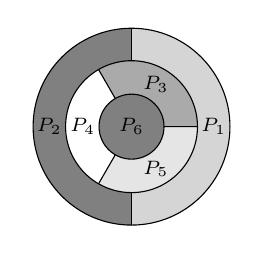
\begin{tikzpicture}[scale = 1.25]
\fill[gray!33] (0,1) arc (90:-90:1) -- cycle;
\fill[gray!100] (0,1) arc (90:270:1) -- cycle;
\draw (0,0) circle (1);
\draw (0,-1) -- (0,1);
\fill[gray!67] (0,0) -- (0:0.67) arc (0:120:0.67) -- cycle;
\fill[gray!0] (0,0) -- (120:0.67) arc (120:240:0.67) -- cycle;
\fill[gray!20] (0,0) -- (240:0.67) arc (240:360:0.67) -- cycle;
\draw (0,0) circle (0.67);
\draw (0,0) -- (0:0.67) -- (0,0) -- (120:0.67) -- (0,0) -- (240:0.67) -- cycle;
\fill[gray!100] (0,0) circle (0.33);
\draw (0,0) circle (0.33);
\node at (0.835,0) {\scriptsize $P_1$};
\node at (-0.835,0) {\scriptsize $P_2$};
\node at (60:0.495) {\scriptsize $P_3$};
\node at (180:0.495) {\scriptsize $P_4$};
\node at (300:0.495) {\scriptsize $P_5$};
\node at (0:0) {\scriptsize $P_6$};
\end{tikzpicture}
\caption{Partition of $\Omega$.}
\label{fig:partition3}
\end{figure}
We explore the quality of the reconstructions given by the algorithm suggested by Corollary \ref{cr:multipledescent}.
Starting at the constant conductivity $\tau(j)=1.8$, we optimize the coordinates of $\tau$ according to the functionals $c_1 = (1,1,0,0,0,0)$, $c_2 = (0,0,1,1,1,0,0)$ and $c_3 = (0,0,0,0,0,1)$.
Each functional was optimized $200$ epochs by keeping the first coordinates at their values found in previous steps and the last components fixed at $1.8$.
If $\tau_n$ is the reconstruction at epoch $n$, Figure \ref{fig:coordinatedescent} shows the values $\tau_n(j)-\sigma(j)$ for $j = 1,\dots,J$.
Computational details are similar to those described in Example \ref{ex:ones}.
\begin{figure}[H]
\centering
\input{figures/coordinatedescent}
\caption{Epoch $k$ v.s. difference between components of $\tau_k$ and $\sigma$.}
\label{fig:coordinatedescent}
\end{figure}
The final iterate of the process is $\tau = (1.04, 1.53, 1.10, 0.70, 0.79, 2.11)$ which yields the error vector $\tau - \sigma = (0.04,0.03,-0.15,-0.05,-0.11,0.61)$.
As expected, the further the pixel $P_j$ is into the domain the greater the discrepancy between $\tau(j)$ and $\sigma(j)$.
Indeed, in addition to numerical errors, at each stage one source of error is the discretization error described in Example \ref{ex:ones}.
Moreover, the errors keep propagating at each one of the stages $l = 1,2,\dots,\max_j d(j)$.
\end{example}

If the functionals $c_1,\dots,c_m$ are defined as $c_l(j)=1$ if $d(j)=l$ and $0$ otherwise then \ref{cr:multipledescent} states that
$$ \face_{c_m}\left(\face_{c_{m-1}}\left(\dots \left(\face_{c_1}\left(K_\sigma\right)\right)\right)\right) = \{\sigma\}$$
where $K_\sigma = \{\tau\in K : \Lambda(\tau)\leq\Lambda(\sigma)\}$.
The next conjecture is based on the fact, that if $K'$ is a polytope and $c_1,\dots,c_m$ are functionals, studying the normal fan to $K'$ yields an $\epsilon>0$ such that 
$$ \face_{c_m}\left(\face_{c_{m-1}}\left(\dots \left(\face_{c_1}\left(K'\right)\right)\right)\right) = \face_{c_1+\epsilon c_2 + \dots + \epsilon^{m-1}c_m}\left(K'\right).$$
\begin{conjecture}\label{cj:normalfan}
There exists an $\epsilon > 0$ such that for each $\sigma\in K$ the unique minimizer of 
\begin{align*}
&\textup{min}\;\; \sum_{j}\epsilon^{d(j)-1}\tau(j) \\
&\textup{subject to }\; \tau \in K \\
&\phantom{\textup{subject to }\;} \Lambda(\tau) \leq \Lambda(\sigma)
\end{align*}
is $\sigma$.
In other words, the weight vector can be chosen as $c = \sum_{l}\epsilon^{l-1} c_l$ where $c_l(j)=1$ if $d(j)=l$ and $0$ otherwise (see Figure \ref{fig:normalcone}).
\end{conjecture}

\begin{figure}[H]
\centering
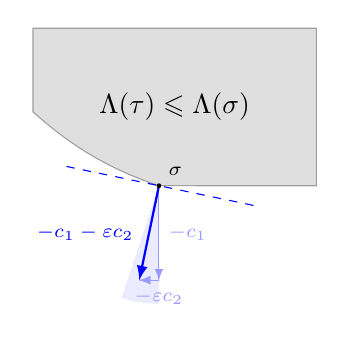
\begin{tikzpicture}[scale = 2, >=latex]
\draw[domain=0.2:1, smooth, variable=\x, gray!75, fill = gray!25] plot ({\x}, {
(-(5*\x-5)+sqrt((5*\x-5)^2+36*\x))/6
}) -- (2,1) -- (2,2) -- (0.2,2) -- cycle;
\node at (1.1,1.5) {$\Lambda(\tau)\leq\Lambda(\sigma)$};
\node[anchor = south west] at (1,1) {\scriptsize $\sigma$};
\fill[blue!8] (1,1) --++ (0,-0.75) arc (-90:-108.43:0.75) -- cycle;
\draw[blue!40, thin, ->] (1,1) --++ (0,-0.6);
\draw[blue!40, thin, ->] (1,0.4) --++ (-0.125,0);
\draw[blue!40, thin, ->] (1,1) --++ (0,-0.6) --++ (-0.125,0);
\draw[blue, thick, ->] (1,1) --++ (-0.125,-0.6);
\node[blue!40, anchor = west] at (1,0.7) {\scriptsize $-c_1$};
\node[blue!40, anchor = north] at (1,0.4) {\scriptsize $-\epsilon c_2$};
\node[blue, anchor = east] at (0.9,0.7) {\scriptsize $-c_1-\epsilon c_2$};
\draw[blue, dashed] ($(1,1)+(0.6,-0.125)$) --++ (-1.2,0.25);
\fill[black] (1,1) circle (0.015);
\end{tikzpicture}
\caption{Normal cone of $K_\sigma$ at $\sigma$.}
\label{fig:normalcone}
\end{figure}

\begin{example}
Consider the partition of the domain $\Omega = B_1(0)\subseteq \mathbb R^2$ shown in Figure \ref{fig:partition} and conductivity $\sigma = (1.0,1.5,1.25,0.75,0.9,1.5)$.
We explore if, by taking the weight vector as suggested in Conjecture \ref{cj:normalfan}, the optimization problem yields (an approximation of) the true conductivity $\sigma$.
The behaviour of the norm $\|\tau_n-\sigma\|$ as a function of $n$ is shown in Figure \ref{fig:normalfanerror} with $\epsilon = \frac1{10}$.
\begin{figure}[H]
\centering
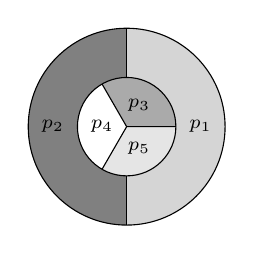
\begin{tikzpicture}[scale = 1.25]
\fill[gray!33] (0,1) arc (90:-90:1) -- cycle;
\fill[gray!100] (0,1) arc (90:270:1) -- cycle;
\draw (0,0) circle (1);
\draw (0,-1) -- (0,1);
\fill[gray!67] (0,0) -- (0:0.5) arc (0:120:0.5) -- cycle;
\fill[gray!0] (0,0) -- (120:0.5) arc (120:240:0.5) -- cycle;
\fill[gray!20] (0,0) -- (240:0.5) arc (240:360:0.5) -- cycle;
\draw (0,0) circle (0.5);
\draw (0,0) -- (0:0.5) -- (0,0) -- (120:0.5) -- (0,0) -- (240:0.5) -- cycle;
\node at (0.75,0) {\scriptsize $p_1$};
\node at (-0.75,0) {\scriptsize $p_2$};
\node at (60:0.25) {\scriptsize $p_3$};
\node at (180:0.25) {\scriptsize $p_4$};
\node at (300:0.25) {\scriptsize $p_5$};
\end{tikzpicture}
\caption{Partition of $\Omega = B_1(0)$.}
\label{fig:partition}
\end{figure}

\begin{figure}[H]
\centering
\input{figures/normalfanerror}
\caption{Error for iterates $\tau_n$ associated to functional $c = c_1+\epsilon c_2$.}
\label{fig:normalfanerror}
\end{figure}
\end{example}

We now go back to Conjecture \ref{cj:normalfan} and prove some facts pointing in that direction.
\begin{lemma}
Suppose that $d(j)=1$ for each $j=1,2,\dots,J-1$.
Then there exists an $\epsilon > 0$ such that the weight vector can be chosen as $c = (1,\dots,1,\epsilon)$.
That is, if $\sigma\in K$, $\tau\in\mathbb R^J$ and $\Lambda(\tau)\leq\Lambda(\sigma)$ then $c\tau > c\sigma$.
\end{lemma}
\begin{proof}
Let $\sigma$ and $\tau$ as in the statement and note that, as in the proof of Corollary \ref{cr:multipledescent}, we have $\tau(j)\geq\sigma(j)$ for $j=1,\dots,J-1$.
If $\tau(J)\geq\sigma(J)$ it follows trivially that $c\tau\geq c\sigma$ and therefore we assume $\tau(J)<\sigma(J)$.
Let $\displaystyle R > \sup_{\substack{j<J\\ \sigma\in K}}\frac{\|\Lambda'(\sigma)(e_j)\|}{\|\Lambda'(\sigma)(e_J)\|}$, choose $\epsilon = \frac1R$ and define $c = (1,\dots,1,\epsilon)$.
If we suppose by contradiction that $c\tau<c\sigma$ then,
\begin{align}
0 &> \|\Lambda'(\sigma)(e_J)\|R c(\tau-\sigma) \nonumber\\
&= \sum_{j<J}\|\Lambda'(\sigma)(e_J)\| R (\tau(j)-\sigma(j))+ \|\Lambda'(\sigma)(e_J)\|(\tau(J)-\sigma(J)) \label{eq:comparison}\\
&\geq \sum_{j}\|\Lambda'(\sigma)(e_j)\|(\tau(j)-\sigma(j)) \nonumber.
\end{align}
If $f\in L^2_0(\partial\Omega)$ is an eigenvector associated to the smallest eigenvalue $-\|\Lambda'(\sigma)(e_J)\|$ of $\Lambda'(\sigma)(e_J)$ with $\|f\|=1$ then, by convexity,
\begin{align*}
\langle (\Lambda(\tau) - \Lambda(\sigma))f,f\rangle &\geq \langle \Lambda'(\sigma)(\tau-\sigma)f,f\rangle \\
&=\sum_{j < J}(\tau(j)-\sigma(j))\langle\Lambda'(\sigma)(e_j)f,f\rangle - (\tau(J)-\sigma(J))\|\Lambda'(\sigma)(e_J)\| \\
&\geq -\sum_{j < J}(\tau(j)-\sigma(j))\|\Lambda'(\sigma)(e_j)\| - (\tau(J)-\sigma(J))\|\Lambda'(\sigma)(e_J)\| \\
&>0
\end{align*}
where the last inequality follows from \eqref{eq:comparison}.
Finally, this implies that $\Lambda(\tau)-\Lambda(\sigma)$ is not negative semi-definite contradicting $\Lambda(\tau)\leq\Lambda(\sigma)$.
\end{proof}
\begin{lemma}\label{lm:existence}
Let $\sigma\neq\tau\in K$ with $\Lambda(\tau)\leq\Lambda(\sigma)$.
Then there exists $p\in(0,1]$ such that $ \left(\sum_l \epsilon^{l-1}c_l\right) (\tau-\sigma) >0 $ for any $\epsilon\in(0,p]$.
\end{lemma}
\begin{proof}
Take $j\geq 1$ as in Lemma \ref{lm:positivity} and let $l'=d(j)$.
By an argument similar to that of the proof of Corollary \ref{cr:multipledescent}, $\tau(j')\geq\sigma(j')$ for each $j'$ with $d(j')=l'$.
Therefore, if $\delta := \sum_{d(j')=l'}\tau(j')-\sigma(j')> 0$, then
\begin{align*}
\left(\sum_l \epsilon^{l-1}c_l\right) (\tau-\sigma) &= \epsilon^{l'-1}\delta  + \epsilon^{l'}\sum_{l>l'}\epsilon^{l-l'-1}c_l(\tau-\sigma)\\
&\geq\epsilon^{l'-1}\delta - 2bJ\epsilon^{l'}\\
&=\epsilon^{l'-1}\left(\delta - 2bJ\epsilon\right).
\end{align*}
The result follows by setting $\displaystyle p = \frac{\delta}{3bJ}$.
\end{proof}
\todo{Arreglar la prueba o eliminar.}
\begin{proposition}
Fix $\sigma\in K$ and for each $\epsilon>0$ let $\tau_\epsilon\in K$ such that $\Lambda(\tau_\epsilon)\leq \Lambda(\sigma)$ and $c_\epsilon \tau_\epsilon \leq c_\epsilon \sigma$.
Then $\tau_\epsilon\to\sigma$ as $\epsilon \to 0^+$.
\end{proposition}
\begin{proof}
Let $(\epsilon_n)_n$ be a sequence of positive numbers such that $\epsilon_n\to0$ as $n\to\infty$ and $x_n := \tau_{\epsilon_n} - \sigma$ for $\tau_{\epsilon_n}$ as in the statement.
Since $K$ is compact, $(x_n)_n$ contains a convergent subsequence which for simplicity we assume is $(x_n)_n$ itself.
Denote $\displaystyle\lim_{n\to\infty} x_n$ by $x$ and suppose by contradiction that $x\neq 0$.

By Lemma \ref{lm:existence} there exists $p > 0$ sufficiently small such that $x \in H := \left\{ y\in \mathbb R^J : c_p y > 0 \right\}$.
Since $H$ is open, there exists $r>0$ such that $P := \overline B_r(x) \subseteq H$ with respect to the $\ell_1$ metric.
$P$ is a polytope and therefore has a finite vertex set $V := \text{vert}(P)$.
Again by Lemma \ref{lm:existence} for each $v\in V$ there exists $p_v$ such that $c_\epsilon v > 0$ as long as $\epsilon \in (0,p_v)$.
If $q = \min_{v\in V}p_v$ then for each $v\in V$ we have $c_\epsilon v > 0$ if $\epsilon\in(0,q)$.
Moreover, the same inequality holds for $y\in P = \text{conv}(V)$.

Let $N\in \mathbb N$ such that $\|x_n-x\|_1<r$  and $\epsilon_n < q$ for $n\geqslant N$.
By the previous discussion $c_{\epsilon_n}x_n>0$ since $x_n\in P$, which is a contradiction with the hypothesis $c_{\epsilon_n}x_n\leq 0$.
Therefore $x = 0$ or in other terms, $\lim_{n\to\infty}\tau^{\epsilon_n} =\sigma$.
Finally, as any subsequence of $(\tau_\epsilon)_{\epsilon>0}$ contains a subsequence converging to $\sigma$ it follows that $(\tau_\epsilon)_\epsilon$ itself converges to $\sigma$.
\end{proof}

\printbibliography

\end{document}

